%%%%%%%%%%%%%%%%%%%%%%%%%%%%%%%%%%%%%%%%%%%%%%%%%%%%%%%%%%%
\begin{frame}[fragile]\frametitle{Data Science: What's that?}
\begin{itemize}
\item What comes to mind?
\item Any experience?
\item Whats the expectation?
\end{itemize}
\end{frame}


%%%%%%%%%%%%%%%%%%%%%%%%%%%%%%%%%%%%%%%%%%%%%%%%%%%%%%%%%%%
\begin{frame}[fragile]\frametitle{Man on the Moon - 1969}
\begin{center}
\includegraphics[width=\linewidth,keepaspectratio]{moon}
\end{center}
\end{frame}

%%%%%%%%%%%%%%%%%%%%%%%%%%%%%%%%%%%%%%%%%%%%%%%%%%%%%%%%%%%
\begin{frame}[fragile]\frametitle{Man on the Moon - small data}
\begin{itemize}
\item Computer Program: FORTRAN, 64kb on 2kb RAM. 
\item Must work 1st time!!!
\item Men must return home!!!
\end{itemize}
\end{frame}

%%%%%%%%%%%%%%%%%%%%%%%%%%%%%%%%%%%%%%%%%%%%%%%%%%%%%%%%%%%
\begin{frame}[fragile]\frametitle{Man on the Moon - Big data}
\begin{itemize}
\item SkyDive Stratos 2012: Tens of Gigabytes
\item We live in Crazy Times!!
\item The Era of Data
\end{itemize}
\end{frame}

%%%%%%%%%%%%%%%%%%%%%%%%%%%%%%%%%%%%%%%%%%%%%%%%%%%%%%%%%%%
\begin{frame}[fragile]\frametitle{Data Science: New?}

\begin{itemize}
\item Data Analysis has been around for a while
\item Data Science : Computational Statistics
\item And Statistics has been around for centuries
\item Old Wine in New Bottle?
\end{itemize}
\end{frame}

%%%%%%%%%%%%%%%%%%%%%%%%%%%%%%%%%%%%%%%%%%%%%%%%%%%%%%%%%%%
\begin{frame}[fragile]\frametitle{Newer milestones}
\begin{itemize}
\item Fisher, 1935: ANOVA (analysis of variance), also credited with quote ``correlation does not imply causation'' - lifetime pipe smoker, he rediculed papers showing a link between smoking and cancer. 
\item Deming, 1939: Quality control, Statistical Sampling
\item Luhn, 1958: Information Retrival, use of data and text in business decision making
\end{itemize}
\end{frame}

%%%%%%%%%%%%%%%%%%%%%%%%%%%%%%%%%%%%%%%%%%%%%%%%%%%%%%%%%%%
\begin{frame}[fragile]\frametitle{Newer milestones}
\begin{itemize}
\item Tukey, 1977: Exploratory data analsysis, led to S, S+ and R
\item Dresner, 1989:  Modern proponent of BI
\item Tom Mitchell's ML book, 1997: Still a best-seller
\end{itemize}
\end{frame}

%%%%%%%%%%%%%%%%%%%%%%%%%%%%%%%%%%%%%%%%%%%%%%%%%%%%%%%%%%%
\begin{frame}[fragile]\frametitle{Then came internet}
Access to more and more data
\begin{itemize}
\item Google, 1996: Started as a research project by Larry Page and Sergey Brin, PhD students at Stanford.
\item Data Deluge, 2010: Exponential growth in data
\end{itemize}
\end{frame}

%%%%%%%%%%%%%%%%%%%%%%%%%%%%%%%%%%%%%%%%%%%%%%%%%%%%%%%%%%%
\begin{frame}[fragile]\frametitle{Data All Around}
Lots of data is being collected and warehoused 

\begin{itemize}
\item Web data, e-commerce
\item Financial transactions, bank/credit transactions
\item Online trading and purchasing
\item Social Network
\end{itemize}
\end{frame}

%%%%%%%%%%%%%%%%%%%%%%%%%%%%%%%%%%%%%%%%%%%%%%%%%%%%%%%%%%%
\begin{frame}[fragile]\frametitle{How Much Data Do We have?}
\begin{itemize}
\item Google processes 20 PB a day (2008)
\item Facebook has 60 TB of daily logs
\item eBay has 6.5 PB of user data + 50 TB/day (5/2009)
\item 1000 genomes project: 200 TB
\end{itemize}
\end{frame}

%%%%%%%%%%%%%%%%%%%%%%%%%%%%%%%%%%%%%%%%%%%%%%%%%%%%%%%%%%%
\begin{frame}[fragile]\frametitle{Current Usage}
\begin{center}
\includegraphics[width=\linewidth,keepaspectratio]{datadeluge}
\end{center}
\end{frame}

%%%%%%%%%%%%%%%%%%%%%%%%%%%%%%%%%%%%%%%%%%%%%%%%%%%%%%%%%%%
\begin{frame}[fragile]\frametitle{What To Do With These Data?}
\begin{itemize}
\item Data warehousing : Aggregation and Statistics 
\item Indexing, Searching, and Querying
\item Knowledge discovery
\end{itemize}
\end{frame}

%%%%%%%%%%%%%%%%%%%%%%%%%%%%%%%%%%%%%%%%%%%%%%%%%%%%%%%%%%%%
%\begin{frame}[fragile]\frametitle{The potential}
%New models are estimating which cities are most at risk for spread of the Ebola virus.
%
%\begin{center}
%\includegraphics[width=0.5\linewidth,keepaspectratio]{ebola}
%\end{center}
%\end{frame}


%%%%%%%%%%%%%%%%%%%%%%%%%%%%%%%%%%%%%%%%%%%%%%%%%%%%%%%%%%%
\begin{frame}[fragile]\frametitle{Whats happening?}
Predicting political champagne and election Outcome.
\begin{center}
\includegraphics[width=0.6\linewidth,keepaspectratio]{elections}
\end{center}
\end{frame}

%%%%%%%%%%%%%%%%%%%%%%%%%%%%%%%%%%%%%%%%%%%%%%%%%%%%%%%%%%%
\begin{frame}[fragile]\frametitle{Whats happening?}
\begin{itemize}
\item Transaction Databases: Recommender systems (NetFlix), Fraud Detection (Security and Privacy)
\item Wireless Sensor Data: Smart Home, Real-time Monitoring, Internet of Things
\item Text Data, Social Media Data: Product Review and Consumer Satisfaction (Facebook, Twitter, LinkedIn), E-discovery
\end{itemize}
\end{frame}

%
%%%%%%%%%%%%%%%%%%%%%%%%%%%%%%%%%%%%%%%%%%%%%%%%%%%%%%%%%%%%
%\begin{frame}[fragile]\frametitle{Whats happening?}
%\begin{itemize}
%\item Software Log Data: Automatic Trouble Shooting (Splunk)
%\item Genotype and Phenotype Data: Epic, 23andme, Patient-Centered Care, Personalized Medicine
%\item All human generated information up to 2003 is 5 exabytes. Same amount of data was generate every 2 days in 2011 and would be every 10 min NOW.
%\end{itemize}
%\end{frame}

%%%%%%%%%%%%%%%%%%%%%%%%%%%%%%%%%%%%%%%%%%%%%%%%%%%%%%%%%%%
\begin{frame}[fragile]\frametitle{``Data is the New Oil''}
\begin{itemize}
\item ``Data is the new oil'': Clive Huby, 2006, was embraced by the World Economic Forum in a 2011 report
\item  Data is just like crude oil. 
\end{itemize}
\begin{center}
\includegraphics[width=0.7\linewidth,keepaspectratio]{oil}
\end{center}
\end{frame}

%%%%%%%%%%%%%%%%%%%%%%%%%%%%%%%%%%%%%%%%%%%%%%%%%%%%%%%%%%%
\begin{frame}[fragile]\frametitle{``Data is the New Oil''}
\begin{itemize}
\item It's valuable, but if unrefined it cannot really be used. 
\item It has to be changed into gas, plastic, chemicals, etc to create a valuable entity that drives profitable activity
\item So, it must data be broken down, analyzed for it to have value.
\end{itemize}
\end{frame}

%%%%%%%%%%%%%%%%%%%%%%%%%%%%%%%%%%%%%%%%%%%%%%%%%%%%%%%%%%%
\begin{frame}[fragile]\frametitle{`The Science [and art] of}
\begin{itemize}
\item Discovering what we don't know from data
\item Obtaining actionable insights
\item Predictions
\item Communicating relevant business stories
\item Building confidence in the business decisions.
\end{itemize}
\end{frame}



%%%%%%%%%%%%%%%%%%%%%%%%%%%%%%%%%%%%%%%%%%%%%%%%%%%%%%%%%%%
\begin{frame}[fragile]\frametitle{Characteristics of Data}
\begin{itemize}
\item Volume: Size
\item Velocity: Speed of generation, consumption
\item Variety: Data Types
\item Veracity: Uncertainness, Quality
\end{itemize}
\end{frame}

%%%%%%%%%%%%%%%%%%%%%%%%%%%%%%%%%%%%%%%%%%%%%%%%%%%%%%%%%%%
\begin{frame}[fragile]\frametitle{What is Data Science?}
\begin{center}
{\em ``Data Science is the science which uses computer science, statistics and machine learning, visualization and human-computer interactions to collect, clean, integrate, analyze, visualize, interact with data to create data products.''}
\end{center}
\end{frame}



%%%%%%%%%%%%%%%%%%%%%%%%%%%%%%%%%%%%%%%%%%%%%%%%%%%%%%%%%%%
\begin{frame}[fragile]\frametitle{What is Data Science?}
\begin{itemize}
\item An area that manages, manipulates, extracts, and interprets knowledge from tremendous amount of data
\item Data science (DS) is a multidisciplinary field of study with goal to address the challenges in big data
\item Data science principles apply to all data : big and small

\end{itemize}
\end{frame}


%%%%%%%%%%%%%%%%%%%%%%%%%%%%%%%%%%%%%%%%%%%%%%%%%%%%%%%%%%%
\begin{frame}[fragile]\frametitle{Goal of Data Science}
\begin{center}
{\em `Turn data into data products''}

\includegraphics[width=\linewidth,keepaspectratio]{datajiu}

\tiny{(Reference: Big Data [sorry] \& Data Science: What Does a Data Scientist Do? - Data Science London)}
\end{center}
\end{frame}

%%%%%%%%%%%%%%%%%%%%%%%%%%%%%%%%%%%%%%%%%%%%%%%%%%%%%%%%%%%
\begin{frame}[fragile]\frametitle{Multi Disciplinary}
\begin{itemize}
\item Computer Science: Algorithms, Databases, AI
\item Mathematics and Statistics.

\end{itemize}
\end{frame}

%%%%%%%%%%%%%%%%%%%%%%%%%%%%%%%%%%%%%%%%%%%%%%%%%%%%%%%%%%%
\begin{frame}[fragile]\frametitle{A Visual Definition}
\begin{center}
\includegraphics[width=0.65\linewidth,keepaspectratio]{vizdef}
\end{center}
\end{frame}

%%%%%%%%%%%%%%%%%%%%%%%%%%%%%%%%%%%%%%%%%%%%%%%%%%%%%%%%%%%
\begin{frame}[fragile]\frametitle{Big Data and Data Science}
\begin{center}
{\em `` \ldots the sexy job in the next 10 years will be statisticians'' - Hal Varian, Google Chief Economist}
\end{center}
\end{frame}

%%%%%%%%%%%%%%%%%%%%%%%%%%%%%%%%%%%%%%%%%%%%%%%%%%%%%%%%%%%
\begin{frame}[fragile]\frametitle{Big Data and Data Science}
\begin{center}
{\em `` The U.S. will need 140,000-190,000 predictive analysts and 1.5 million managers/analysts by 2018'' - McKinsey Global Institute's June 2011}
\end{center}
\end{frame}

%%%%%%%%%%%%%%%%%%%%%%%%%%%%%%%%%%%%%%%%%%%%%%%%%%%%%%%%%%%
\begin{frame}[fragile]\frametitle{Real Life Examples}
Companies learn your secrets, shopping patterns, and preferences

\begin{center}
{\em ``For example, can we know if a woman is pregnant, even if she doesn't want us to know? 
'' - ``How Companies Learn Your Secrets'' NYT, by Charles Duhigg, February 16, 2012
}
\end{center}
\end{frame}

%%%%%%%%%%%%%%%%%%%%%%%%%%%%%%%%%%%%%%%%%%%%%%%%%%%%%%%%%%%
\begin{frame}[fragile]\frametitle{What did Target Do?}
Mining of data on shopping patterns

\begin{itemize}
\item Specific products purchased
\item Combination of products purchased
\item Combined with demographic and other data
\end{itemize}
\end{frame}


%%%%%%%%%%%%%%%%%%%%%%%%%%%%%%%%%%%%%%%%%%%%%%%%%%%%%%%%%%%
\begin{frame}[fragile]\frametitle{Data Scientists}
They find stories, extract knowledge. They are not mere reporters.
\begin{center}
\includegraphics[width=0.9\linewidth,keepaspectratio]{datasc}
\end{center}
\tiny{(Reference: https://i.pinimg.com/736x/18/54/3a/ 18543ab2d33d9675c4b1f92ec7014be9-- tops-online-courses.jpg)}
\end{frame}

%%%%%%%%%%%%%%%%%%%%%%%%%%%%%%%%%%%%%%%%%%%%%%%%%%%%%%%%%%%
\begin{frame}[fragile]\frametitle{Data Scientists}
Josh Wills, 2012
\begin{center}
\includegraphics[width=0.8\linewidth,keepaspectratio]{josh}
\end{center}
\end{frame}

%%%%%%%%%%%%%%%%%%%%%%%%%%%%%%%%%%%%%%%%%%%%%%%%%%%%%%%%%%%
\begin{frame}[fragile]\frametitle{What do Data Scientists do?}
\begin{lstlisting}
	class DataScientist {
		Is skeptical, curious
		Knows  Statistics and Linear Algebra
		Knows Mahcine Learning
		Cleans data
		Runs experiments
		Good at coding, hacking
		Can tell good business stories
		Has domain knowledge
	}
\end{lstlisting}
\end{frame}

%%%%%%%%%%%%%%%%%%%%%%%%%%%%%%%%%%%%%%%%%%%%%%%%%%%%%%%%%%%
\begin{frame}[fragile]\frametitle{How to be a Data Scientist}
\begin{itemize}
\item Background in Mathematics  esepcially Statistics.
\item Solid Programming Skills (R, Python, Julia, SQL)
\item Machine Learning
\end{itemize}
\end{frame}

%%%%%%%%%%%%%%%%%%%%%%%%%%%%%%%%%%%%%%%%%%%%%%%%%%%%%%%%%%%
\begin{frame}[fragile]\frametitle{AI Hierarchy of Needs}

\begin{center}
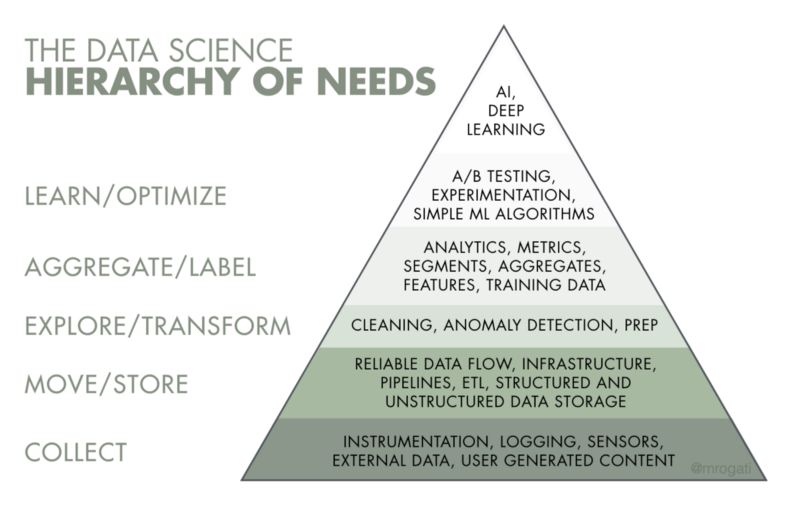
\includegraphics[width=0.9\linewidth,keepaspectratio]{AIhierarchyofneeds}

Data engineering falls into levels 2 and 3 primarily
\end{center}

{\tiny (Ref: What is Data Engineering and Why Is It So Important? - Nathan Black)}

\end{frame}

%%%%%%%%%%%%%%%%%%%%%%%%%%%%%%%%%%%%%%%%%%%%%%%%%%%%%%%%%%%
\begin{frame}[fragile]\frametitle{Data Engineer Vs Data Scientist}

\begin{center}
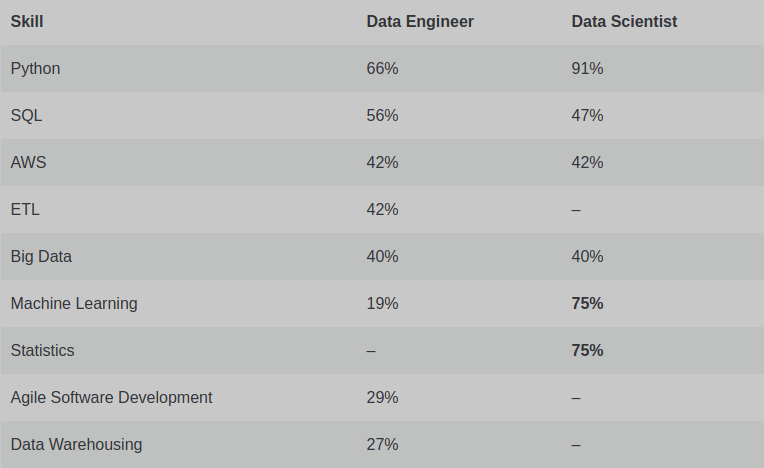
\includegraphics[width=\linewidth,keepaspectratio]{datascvsdataeng}

\end{center}

{\tiny (Ref: Frequency of Skill Appearing in Job Ads, Data Source: IT Jobs Watch (CC BY-NC-SA 4.0))}

\end{frame}


%%%%%%%%%%%%%%%%%%%%%%%%%%%%%%%%%%%%%%%%%%%%%%%%%%%%%%%%%%%
\begin{frame}[fragile]\frametitle{Data engineering activities}

\begin{center}
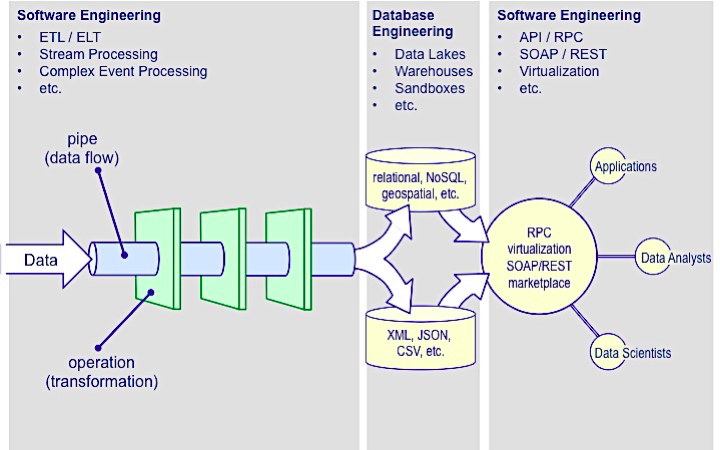
\includegraphics[width=\linewidth,keepaspectratio]{dataengineeringactivities}

\end{center}

{\tiny (Ref: What is Data Engineering and Why Is It So Important? - Nathan Black)}

\end{frame}

%%%%%%%%%%%%%%%%%%%%%%%%%%%%%%%%%%%%%%%%%%%%%%%%%%%%%%%%%%%
\begin{frame}[fragile]\frametitle{Data engineering skills}
\begin{itemize}
\item Architecting distributed systems
\item Creating reliable pipelines
\item Combining data sources
\item Architecting data stores
\item Collaborating with data science teams and building the right solutions for them
\end{itemize}
\end{frame}

%%%%%%%%%%%%%%%%%%%%%%%%%%%%%%%%%%%%%%%%%%%%%%%%%%%%%%%%%%%
\begin{frame}[fragile]\frametitle{Data Engineering Roles}
\begin{itemize}
\item Generalist: small team
\item Pipeline-centric:medium size teams, transform data into a useful format for analysis.
\item Database-centric: large teams, ETL work to get data into warehouses.
\end{itemize}
\end{frame}

% %%%%%%%%%%%%%%%%%%%%%%%%%%%%%%%%%%%%%%%%%%%%%%%%%%%%%%%%%%%
% \begin{frame}[fragile]\frametitle{At the end of the course \ldots}
% Expectation to follow this Water Cooler chat:
% \begin{itemize}
% \item {\em ``We need to reduce features, try correlation plots now''}
% \item {\em ``The model has good precision but low recall''}
% \item {\em ``Which hyperparameters to tune so as to get good F1 score''}
% \item {\em ``Lets not remove all the stopwords as they could be part of NER catchphrase''}
% \end{itemize}
% So, Lets get started \ldots
% \end{frame}

